\documentclass[12pt]{article}
\usepackage[margin=1in]{geometry}
\usepackage{setspace}
\usepackage{graphicx}
\usepackage{booktabs}
\usepackage{tabularx}
\usepackage{array}
\usepackage{amsmath}
\usepackage{float}
\usepackage{hyperref}
\usepackage{longtable}
\usepackage{enumitem}
\usepackage{caption}

\hypersetup{
    colorlinks=true,
    linkcolor=black,
    urlcolor=blue,
    citecolor=black
}

\setlength{\parindent}{0pt}
\setlength{\parskip}{0.5em}
\doublespacing

\begin{document}

\begin{center}
{\LARGE \textbf{A Comparative Backtesting Study of Machine Learning and Rule-Based Trading Strategies in Cryptocurrency Markets}}\\[1.5em]

\begingroup
\singlespacing
\begin{tabular}{ll}
\textbf{Group Member} & \textbf{Matriculation Number} \\
\midrule
Lau Ming Jie & A0272632H \\
Loo Wen Wen & A0259594J \\
Low Ruo Fei Evie & A0259605X \\
Wilbert Christopher Kurniawan & A0282267X \\
Wu Xuande & A0287897W \\
\end{tabular}
\endgroup

\vspace{1em}
GitHub Repository: \url{https://github.com/xdewu0508/QF4211Project}
\end{center}

\section{Introduction}

Cryptocurrency markets trade continuously, undergo large regime shifts, and lack the conventional valuation anchors that often guide trading in equities or bonds. In such markets, technical trading rules based on price, volume, and momentum remain common, while machine-learning models promise greater flexibility in capturing non-linear and sequential structure. The practical question, however, is not whether a model can generate directional predictions in isolation, but whether those signals survive a realistic backtest once transaction costs and portfolio turnover are taken seriously.

This study therefore asks a focused empirical question: under a common hourly backtesting framework with transaction costs, do machine-learning strategies outperform rule-based technical strategies and passive buy-and-hold benchmarks across BTC, ETH, XRP, and SOL? We evaluate four machine-learning models (Logistic Regression, XGBoost, LightGBM, and GRU), two traditional rule-based strategies (SMA and RSI), and a buy-and-hold benchmark under long-only, short-only, and long-short structures.

Our contribution is a cost-aware, cross-asset comparison rather than a claim that machine learning consistently dominates cryptocurrency trading. The results show that long-only strategies are the most stable active structure, but that transaction costs substantially erode performance. Machine-learning models provide pockets of improvement in selected settings, yet they do not deliver robust, statistically significant outperformance over simpler alternatives within the current evaluation design.

\section{Literature Review}

\subsection{Traditional Technical Trading in Cryptocurrency Markets}

Because cryptocurrency assets do not generate cash flows or dividends, market participants often rely on technical indicators such as moving averages and RSI to form trading signals. Prior work has shown that technical rules can outperform passive exposure in some cryptocurrency settings, but the results are highly sensitive to parameter choice, market state, and transaction-cost assumptions. Another gap in the literature is that many studies emphasize long-only designs, leaving the behavior of short-only and long-short structures less examined.

\subsection{Machine Learning in Trading}

Machine-learning approaches have become increasingly common in cryptocurrency forecasting, with linear models, boosted trees, and recurrent neural networks all appearing in the literature. These models can capture non-linear interactions and temporal dependencies that simple rule-based systems may miss. At the same time, the literature repeatedly warns that strong in-sample performance does not guarantee robust out-of-sample trading gains, especially in non-stationary markets with substantial execution frictions.

\subsection{Positioning Our Study}

This project sits between replication and extension. We adopt the hourly, feature-based cryptocurrency prediction setting of the reference paper, but expand the comparison across four assets and multiple strategy structures while explicitly incorporating a \texttt{0.035\%} transaction fee per unit position change. The study prioritizes economic evaluation rather than raw classification quality: strategies are compared using cumulative return, drawdown, turnover, trading frequency, and Sharpe-style metrics. At the same time, our claims remain deliberately scoped to the submitted evaluation design rather than to all market regimes or all possible crypto trading environments.

\section{Data Description and Preprocessing}

\subsection{Data Source and Assets}

The dataset is drawn from Binance public hourly candlestick files for four liquid USDT spot pairs: BTC/USDT, ETH/USDT, XRP/USDT, and SOL/USDT. These assets were selected to provide a mix of large-cap and higher-beta behavior while keeping the market venue, fee assumptions, and data structure consistent across the analysis.

\subsection{Sample Period}

The raw hourly files span approximately five years, from January 2021 to December 2025. After forward-return alignment, the canonical notebook works with \texttt{43,808} usable hourly observations per asset. This window contains multiple market phases, including the 2021 bull market, the 2022 drawdown, the 2023 recovery, the 2024 ETF-driven institutional surge, and the volatile conditions late in 2025. That breadth makes the sample more informative than a single-regime window, but it does not by itself establish regime-invariant robustness because the final evaluation still relies on one fixed chronological split.

Hourly data were retained to remain aligned with the reference paper and to preserve an intraday decision horizon, while still being coarse enough to avoid the extreme noise and execution burden of sub-hourly strategies. Even so, hourly signals remain noisy and turnover-sensitive, which is important when interpreting the final results.

\subsection{Data Construction}

We construct four feature sets. \texttt{ohlc\_raw} uses open, high, low, close, volume, trade count, and cyclical hour terms. \texttt{candle\_raw} replaces the raw OHLC block with candlestick body and shadow representations while retaining volume, trade count, and cyclical terms. \texttt{ohlc\_extended} and \texttt{candle\_extended} augment the corresponding raw sets with technical indicators including SMA, RSI, MACD line and histogram, Williams \%R, stochastic oscillator, and MFI. All features are lagged so that only information available at or before the current hour is used when generating a trade for the next-hour open entry and the following-hour open exit.

\subsection{Train / Validation / Test Split}

Each asset is divided chronologically into \texttt{50\%} training, \texttt{25\%} validation, and \texttt{25\%} testing. Under the current notebook logic this yields \texttt{21,902} training rows, \texttt{10,950} validation rows, and \texttt{10,952} test rows per asset after the forward-return alignment and split-boundary trimming are applied. This design avoids look-ahead bias and provides a clean held-out test window under one common protocol. However, it is still a single realised historical partition. The resulting evidence should therefore be interpreted as out-of-sample performance for this fixed split, not as proof that the same model rankings will persist under rolling or walk-forward re-estimation across different market regimes.

\section{Methodology and Model Explanation}

\subsection{Prediction Labelling}

The predictive task is framed as two binary classification problems built on the next-hour open-to-open log return. The strategy observes the current feature vector, enters at the next hour’s open if a threshold is triggered, and exits one hour later at the following open. We define:

\begin{itemize}
    \item \texttt{label\_up = 1} when the next-hour open-to-open log return is positive,
    \item \texttt{label\_down = 1} when the next-hour open-to-open log return is negative.
\end{itemize}

This dual-labelling design allows long-only, short-only, and long-short trading structures to be implemented consistently across both machine-learning and rule-based strategies.

Class imbalance is limited in the submitted chronological split. Across the four training sets, the share of \texttt{label\_up = 1} ranges from \texttt{49.2\%} to \texttt{50.6\%}, while the share of \texttt{label\_down = 1} ranges from \texttt{48.3\%} to \texttt{49.6\%}; the residual corresponds to zero-return hours. Severe one-sided label dominance is therefore not the main driver of the reported results.

\subsection{Strategy Families}

\subsubsection{Buy-and-Hold Benchmark}

Buy-and-hold maintains a constant long position over the full test period and serves as the passive benchmark. In the \texttt{with\_cost} setting, the benchmark incurs the one-time initial entry cost implied by moving from zero exposure to a fully invested long position.

\subsubsection{Rule-Based Technical Heuristics}

SMA and RSI serve as rule-based benchmarks. For SMA, short windows of \texttt{5}, \texttt{10}, \texttt{20}, and \texttt{30} hours are paired with long windows of \texttt{50}, \texttt{100}, \texttt{150}, and \texttt{200} hours. For RSI, windows of \texttt{7}, \texttt{14}, and \texttt{21} hours are tested. Each rule produces a continuous score, which is then mapped through the same validation and thresholding pipeline used for the machine-learning strategies. The long-only, short-only, and long-short structures therefore apply to SMA and RSI as well, rather than only to the ML models.

\subsubsection{Machine-Learning Models}

Four machine-learning models are evaluated. Logistic Regression provides a linear probability baseline. XGBoost and LightGBM represent tree-based ensembles that capture non-linear feature interactions. GRU is the sequential model, using a 24-hour lookback window to learn temporal dependencies in the input features. The GRU architecture used in the notebook is a compact recurrent model with a 16-unit GRU layer followed by a dense layer, dropout, and a sigmoid output.

\subsection{Backtesting Framework}

Backtests are executed under both \texttt{no\_cost} and \texttt{with\_cost} regimes. The \texttt{with\_cost} setting applies a transaction cost of \texttt{0.035\%} per unit position change. Opening or closing a unit position therefore costs \texttt{0.035\%}, while directly flipping from long to short costs \texttt{0.07\%}. This design penalizes high-turnover strategies and makes it possible to separate raw predictive opportunity from economic viability after friction.

All portfolios are evaluated from a normalized initial capital of \texttt{1}. Positions are unit-scaled (\texttt{+1} long, \texttt{0} flat, \texttt{-1} short), so capital utilisation changes through time-in-market rather than through leverage sizing; this is why turnover and trading frequency are reported alongside the return-based metrics.

\subsection{Evaluation Metrics and Feasibility Rules}

Following the reference paper, the main benchmark is built from compounded signal returns rather than annualized hourly returns. Using the paper's notation,
\[
\text{Total Return} = \prod_{i=1}^{N}(1 + R_i S_i)
\]
\[
\text{Average Return} = \frac{\text{Total Return}}{\sum_{i=1}^{N} S_i}
\]
\[
\text{Sharpe Ratio} = \frac{\text{Average Return}}{\text{Standard Deviation of Return}}
\]
where \(R_i\) is the realized one-period return and \(S_i \in \{0,1\}\) indicates whether a signal is active at time \(i\). Operationally, the notebook applies this same compounded-return logic to the realized active net-return sequence: if \(r_j\) denotes the active signal returns, the implementation uses \((\prod_{j=1}^{N_{\text{sig}}}(1+r_j)-1)/N_{\text{sig}}\) in the numerator and divides by the standard deviation of the signal-return sequence. This remains the headline Sharpe metric in the summary tables.

We also report annualized Sharpe as a secondary diagnostic:
\[
\text{Annualized Sharpe} =
\frac{\mu(r_t - r_f / 8760)}{\sigma(r_t - r_f / 8760)} \sqrt{8760}
\]
where \(r_t\) denotes hourly net returns and \(r_f = 0\) in the submitted implementation.

Thresholds are selected on the validation set using a precision-first rule subject to feasibility constraints. Specifically, a candidate threshold must generate at least \texttt{20} trades, a signal ratio of at least \texttt{0.2\%}, and recall of at least \texttt{1\%} before it is considered feasible. Among feasible thresholds, precision is prioritized, with recall and validation Sharpe used only as secondary tie-breakers. This is a deliberate high-confidence signal-selection design: the goal is first to filter noisy trades, then to judge the resulting strategy economically out of sample. The report’s main tables, grouped statistical tests, and representative graphs all focus on these feasible configurations, while infeasible cases are retained separately in diagnostic exports.

\section{Model Performance Evaluation and Analysis}

\subsection{Overall Performance Comparison}

The appendix now contains the supporting tables so that the main body can focus on interpretation. Appendix~\ref{app:tables} includes the overall feasible-performance summary, the buy-and-hold benchmark table, model-family comparisons, grouped representation tables, and the significant grouped-bootstrap results that support the discussion below.

The headline result is clear: long-only is the strongest active structure in the current experiment, but even long-only becomes far less attractive once fees are included. Long-short and short-only strategies deteriorate sharply under costs because their higher turnover compounds the fee burden. This directly answers the research question: machine learning does not deliver a broad, cost-robust victory over simpler strategies in this setting.

Buy-and-hold also remains a difficult benchmark. On the test set, the benchmark annualized Sharpe ratios are \texttt{0.82} for BTC, \texttt{0.53} for ETH, \texttt{1.40} for XRP, and \texttt{0.25} for SOL. Some active configurations do produce positive absolute performance in selected asset-strategy combinations, but there is little evidence that active trading consistently dominates passive exposure across assets once the full set of frictions is imposed.

\subsection{Impact of Transaction Costs}

The \texttt{no\_cost} versus \texttt{with\_cost} comparison shows that transaction costs are not a secondary detail; they are central to the ranking of strategies. Averaging across feasible configurations, long-only cumulative return falls from \texttt{0.2397} to \texttt{-0.1065} when costs are introduced. The effect is more severe for long-short and short-only designs because their average trade counts are much larger. Long-short strategies average roughly \texttt{2,144} trades, compared with \texttt{1,068} for long-only.

This pattern also explains why models that look moderately attractive in gross terms often fail to survive in net terms. More complex strategies can generate more signals, but signal volume is not automatically a virtue when each position change incurs a cost.

\subsection{Model-Level Comparison}

At the family level, ML strategies are somewhat stronger than the rule-based benchmarks in the frictionless setting: the average feasible test Sharpe is \texttt{0.0275} for ML models versus \texttt{-0.0012} for rule-based strategies. After costs, however, the gap narrows materially, with ML averaging \texttt{-0.0004} and rule-based strategies averaging \texttt{-0.0056}. This is a much weaker conclusion than ``machine learning wins.'' It is more accurate to say that machine-learning models occasionally improve on simple rules in selective cases, but the advantage is fragile and not reliably preserved after costs.

Within the ML group, the current outputs show a split picture rather than a single dominant winner. Across all feasible configurations, Logistic Regression has the highest average test Sharpe among the ML models. In contrast, the all-asset long-only model-average tables are led by GRU in both the no-cost and with-cost settings, while LightGBM is also competitive in several asset-level long-only results. XGBoost is the weakest ML model on average in the submitted configuration. The broader lesson is that extra model complexity does not guarantee more robust out-of-sample trading performance.

\subsection{Feature Representation and Strategy Behaviour}

Within the feasible ML configurations, the grouped all-asset long-only tables favor standard \texttt{ohlc} representations over \texttt{candle} representations in the with-cost setting (test Sharpe \texttt{0.0255} versus \texttt{0.0195}), and they also favor extended feature sets over raw feature sets (\texttt{0.0472} versus \texttt{-0.0024}). This points to a useful distinction: the current notebook does not support the idea that candlestick inputs are broadly superior, but it does support the view that the paper-aligned extended indicators can help in selected settings. Even so, the improvement is economically conditional. The additional indicators can extract directional structure, yet they can also support more active signal generation, which increases turnover and cost exposure. Predictive improvements therefore do not automatically translate into stronger net performance.

The behavior of short-only strategies deserves explicit discussion because the underperformance is consistent. In the with-cost setting, short-only strategies have a negative average Sharpe for every asset, ranging from \texttt{-0.0146} in BTC to \texttt{-0.0345} in ETH. Two mechanisms appear especially important. First, crypto markets over the sample retain enough upside drift that a pure short stance is structurally disadvantaged relative to long-only participation. Second, short-only strategies still trade frequently---about \texttt{1,564} trades on average---so even modest predictive errors are quickly magnified by repeated transaction costs. The issue is therefore not only directional accuracy; it is the combination of weaker underlying market drift and high turnover.

\subsection{Statistical Significance}

The notebook’s main statistical layer uses grouped block-bootstrap tests on feasible ML configurations rather than exhaustive pairwise model-versus-model comparisons. These grouped tests compare \texttt{candle} versus \texttt{ohlc} inputs, \texttt{extended} versus \texttt{raw} feature sets, and \texttt{GRU} versus the rest of the ML set across asset scopes, strategy modes, and cost regimes. In the current rerun, statistical significance is concentrated in a narrow subset of tests rather than appearing broadly across the grid. At the all-asset level, extended features outperform raw features in the with-cost short-only and long-short comparisons, and the \texttt{GRU}-versus-rest contrast is significant in those same with-cost grouped tests. Asset-level significance is similarly selective, with several BTC and ETH with-cost \texttt{GRU} contrasts significant, while the XRP long-only no-cost \texttt{GRU}-versus-rest comparison is significant in the opposite direction. The separate usefulness tests show that some best configurations have positive mean net returns---most clearly SOL long-short in both cost regimes---yet none significantly outperform buy-and-hold. This is important for interpretation: even where some configurations show positive Sharpe ratios or cumulative returns, the evidence of persistent alpha remains narrow and unstable.

\subsection{Equity Curve Analysis}

To avoid crowding the main discussion, the equity-curve figures are moved to Appendix~\ref{app:figures}. The appendix now contains the representative with-cost curves for all four assets across long-only, long-short, and short-only settings, always comparing buy-and-hold with the best feasible configuration per model.

The representative plots reinforce the earlier summary. In BTC, buy-and-hold preserves a comparatively strong upward trajectory while most active strategies remain flatter and struggle to overcome costs. ETH provides a more favorable environment for selected active models, but the gains are still uneven and do not establish sustained dominance over the passive benchmark. These figures are more interpretable than the bundled plots because they isolate the configurations that matter most for the report’s main argument.

\section{Conclusion, Limitations, and Future Work}

\subsection{Conclusion}

This study asks whether machine-learning trading strategies outperform rule-based technical strategies and passive buy-and-hold benchmarks in a cost-aware cryptocurrency backtest. Within the submitted evaluation design, the answer is no in any broad or robust sense. Machine-learning models can improve on simple rule-based strategies in selected settings, especially before costs, but they do not consistently or statistically reliably outperform buy-and-hold once transaction costs are applied.

The strongest active results come from long-only strategies. Short-only and long-short structures are generally too turnover-heavy and fee-sensitive to remain attractive in the current framework. Extended feature sets can improve raw predictive performance, yet their economic gains are often diluted by higher trading activity. GRU sometimes leads the ML group, but the overall evidence does not support the view that more complex models automatically produce better tradable outcomes.

\subsection{Limitations}

Several limitations materially qualify the findings. First, the study uses one fixed chronological train / validation / test split. Although the sample spans multiple market phases, the analysis does not establish whether the observed model rankings would persist under rolling or expanding walk-forward retraining. In a non-stationary market such as cryptocurrency, this is an important limitation.

Second, the predictive target is binary directional classification rather than return regression. This means that a correct prediction on a very small move is treated the same as a correct prediction on a much larger economically important move. The thresholding rules partially mitigate this by filtering for higher-confidence signals, but they do not eliminate the mismatch between directional classification and return magnitude.

Third, the backtest remains stylized. It applies exchange-style transaction fees, but it does not model slippage, execution delay, order-book depth, market impact, borrowing costs for shorting, margin requirements, or liquidation dynamics. As a result, the reported outcomes should be interpreted as conservative relative to a frictionless backtest, but still simpler than a live-trading environment.

Fourth, the study operates at hourly frequency. This preserves an intraday research design and aligns with the reference paper, but it also increases exposure to noise and to turnover-driven cost drag. Lower-frequency strategies may behave differently.

Finally, the submitted version does not include a dedicated explainability analysis or formal feature-selection stage. The engineered features are intentionally paper-aligned, but the project does not yet isolate which indicators contribute most to predictive performance, nor does it test dimensionality-reduction alternatives systematically.

\subsection{Future Work}

The main contribution of the project is comparative and cautionary rather than celebratory. Under one fixed chronological split and a realistic fee model, the practical value of active cryptocurrency trading remains limited, and the margin between machine learning and simpler alternatives is much narrower than headline predictive results might suggest. Future work should test the same families under walk-forward re-estimation, richer backtest frictions, lower-frequency variants, and broader explainability analysis to determine whether any observed advantage survives under stronger robustness checks.

\clearpage
\appendix
\section{Appendix Tables}
\label{app:tables}

The full exported CSV tables remain available under \texttt{result/paper\_tables/}. This appendix reproduces the most important report-facing tables so that the main body can stay interpretation-first.

\begin{table}[H]
\centering
\caption{Average feasible test outcomes across strategy modes.}
\label{tab:appendix_overall_performance}
\begingroup
\singlespacing
\begin{tabular}{lrrrrr}
\toprule
Strategy Mode & Avg. Test Sharpe & Avg. Test Sharpe & Avg. Cum. Return & Avg. Cum. Return & Avg. Number \\
 & (No Cost) & (With Cost) & (No Cost) & (With Cost) & of Trades \\
\midrule
Long-only & 0.0495 & 0.0212 & 0.2397 & -0.1065 & 1068 \\
Long-short & 0.0236 & 0.0006 & 0.1176 & -0.4217 & 2144 \\
Short-only & 0.0005 & -0.0242 & -0.0217 & -0.4057 & 1564 \\
\bottomrule
\end{tabular}
\endgroup
\end{table}

\begin{table}[H]
\centering
\caption{Buy-and-hold benchmark summary on the test set.}
\label{tab:appendix_buyhold}
\begingroup
\singlespacing
\begin{tabular}{lrrrr}
\toprule
Asset & Cumulative Return & Annualized Return & Annualized Sharpe & Maximum Drawdown \\
\midrule
BTC & 0.4010 & 0.3095 & 0.8180 & -0.3476 \\
ETH & 0.1673 & 0.1317 & 0.5303 & -0.6528 \\
XRP & 2.0132 & 1.4163 & 1.4012 & -0.5121 \\
SOL & -0.1723 & -0.1403 & 0.2523 & -0.6606 \\
\bottomrule
\end{tabular}
\endgroup
\end{table}

\begin{table}[H]
\centering
\caption{Average feasible test outcomes by model family.}
\label{tab:appendix_model_family}
\begingroup
\singlespacing
\begin{tabular}{lrrrr}
\toprule
Cost Regime & ML Avg. Sharpe & Rule Avg. Sharpe & ML Avg. Cum. Return & Rule Avg. Cum. Return \\
\midrule
No Cost & 0.0275 & -0.0012 & 0.1369 & -0.0887 \\
With Cost & -0.0004 & -0.0056 & -0.3060 & -0.3537 \\
\bottomrule
\end{tabular}
\endgroup
\end{table}

\begin{table}[H]
\centering
\caption{All-asset long-only model averages, no-cost feasible configurations.}
\label{tab:appendix_table12_nocost}
\begingroup
\singlespacing
\begin{tabular}{lrrrr}
\toprule
Model & Test Sharpe & Test Precision & Test Recall & Test Avg. Return \\
\midrule
GRU & 0.0773 & 0.5885 & 0.0845 & 0.001050 \\
Logistic Regression & 0.0690 & 0.5582 & 0.0386 & 0.000825 \\
LightGBM & 0.0536 & 0.5481 & 0.0725 & 0.000653 \\
SMA & 0.0286 & 0.5239 & 0.0585 & 0.000379 \\
XGBoost & 0.0175 & 0.5176 & 0.1731 & 0.000140 \\
RSI & 0.0069 & 0.5335 & 0.4517 & 0.000069 \\
\bottomrule
\end{tabular}
\endgroup
\end{table}

\begin{table}[H]
\centering
\caption{All-asset long-only model averages, with-cost feasible configurations.}
\label{tab:appendix_table12_withcost}
\begingroup
\singlespacing
\begin{tabular}{lrrrr}
\toprule
Model & Test Sharpe & Test Precision & Test Recall & Test Avg. Return \\
\midrule
GRU & 0.0530 & 0.5885 & 0.0845 & 0.000846 \\
Logistic Regression & 0.0382 & 0.5582 & 0.0386 & 0.000550 \\
SMA & 0.0266 & 0.5239 & 0.0585 & 0.000362 \\
LightGBM & 0.0151 & 0.5481 & 0.0725 & 0.000379 \\
RSI & -0.0026 & 0.5335 & 0.4517 & 0.000001 \\
XGBoost & -0.0128 & 0.5176 & 0.1731 & -0.000098 \\
\bottomrule
\end{tabular}
\endgroup
\end{table}

\begin{table}[H]
\centering
\caption{All-asset long-only input-type comparison, with-cost feasible configurations.}
\label{tab:appendix_table10_withcost}
\begingroup
\singlespacing
\begin{tabular}{lrrrr}
\toprule
Input Type & Test Sharpe & Test Precision & Test Recall & Test Avg. Return \\
\midrule
ohlc & 0.0255 & 0.5629 & 0.0855 & 0.000425 \\
candle & 0.0195 & 0.5425 & 0.0989 & 0.000401 \\
\bottomrule
\end{tabular}
\endgroup
\end{table}

\begin{table}[H]
\centering
\caption{All-asset long-only feature-type comparison, with-cost feasible configurations.}
\label{tab:appendix_table11_withcost}
\begingroup
\singlespacing
\begin{tabular}{lrrrr}
\toprule
Feature Type & Test Sharpe & Test Precision & Test Recall & Test Avg. Return \\
\midrule
extended & 0.0472 & 0.5808 & 0.0579 & 0.000809 \\
raw & -0.0024 & 0.5234 & 0.1264 & 0.000003 \\
\bottomrule
\end{tabular}
\endgroup
\end{table}

\begingroup
\small
\singlespacing
\begin{longtable}{llllrr}
\caption{Significant grouped bootstrap results from the feasible configuration set.}
\label{tab:appendix_sigtests}\\
\toprule
Scope & Strategy Mode & Cost Regime & Test Type & Mean Diff & p-value \\
\midrule
\endfirsthead
\toprule
Scope & Strategy Mode & Cost Regime & Test Type & Mean Diff & p-value \\
\midrule
\endhead
all\_assets & short\_only & with\_cost & extended\_vs\_raw & 0.000027 & 0.0379 \\
all\_assets & short\_only & with\_cost & gru\_vs\_other\_models & 0.000026 & 0.0219 \\
all\_assets & long\_short & with\_cost & extended\_vs\_raw & 0.000037 & 0.0112 \\
all\_assets & long\_short & with\_cost & gru\_vs\_other\_models & 0.000062 & 0.0000 \\
btc & long\_only & with\_cost & gru\_vs\_other\_models & 0.000027 & 0.0002 \\
btc & short\_only & with\_cost & extended\_vs\_raw & 0.000040 & 0.0005 \\
btc & short\_only & with\_cost & gru\_vs\_other\_models & 0.000049 & 0.0000 \\
btc & long\_short & with\_cost & gru\_vs\_other\_models & 0.000068 & 0.0000 \\
eth & long\_short & with\_cost & extended\_vs\_raw & 0.000036 & 0.0420 \\
eth & long\_short & with\_cost & gru\_vs\_other\_models & 0.000068 & 0.0000 \\
xrp & long\_only & no\_cost & gru\_vs\_other\_models & -0.000021 & 0.0236 \\
\bottomrule
\end{longtable}
\endgroup

\section{Appendix Figures}
\label{app:figures}

\subsection{Long-Only With-Cost Equity Curves}

\begin{figure}[H]
\centering
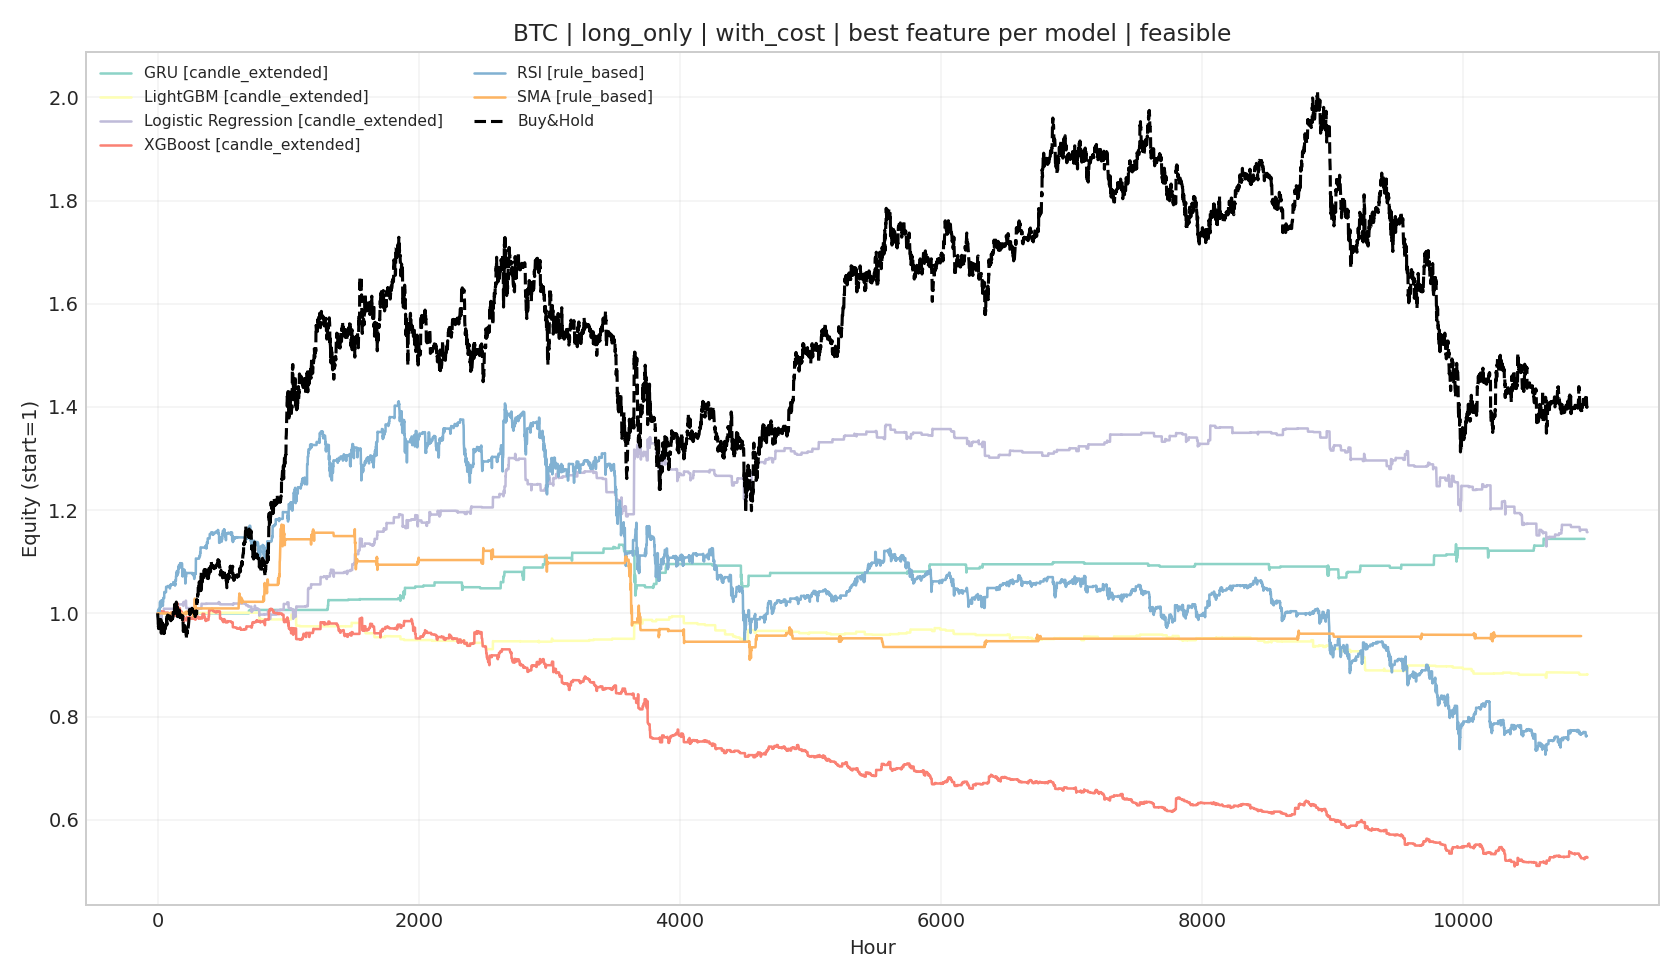
\includegraphics[width=0.9\textwidth]{../result/graph/feasible/BTC/with_cost/long_only/equity_curves_best_feature_per_model_feasible.png}
\caption{BTC long-only equity curves under transaction costs.}
\end{figure}

\begin{figure}[H]
\centering
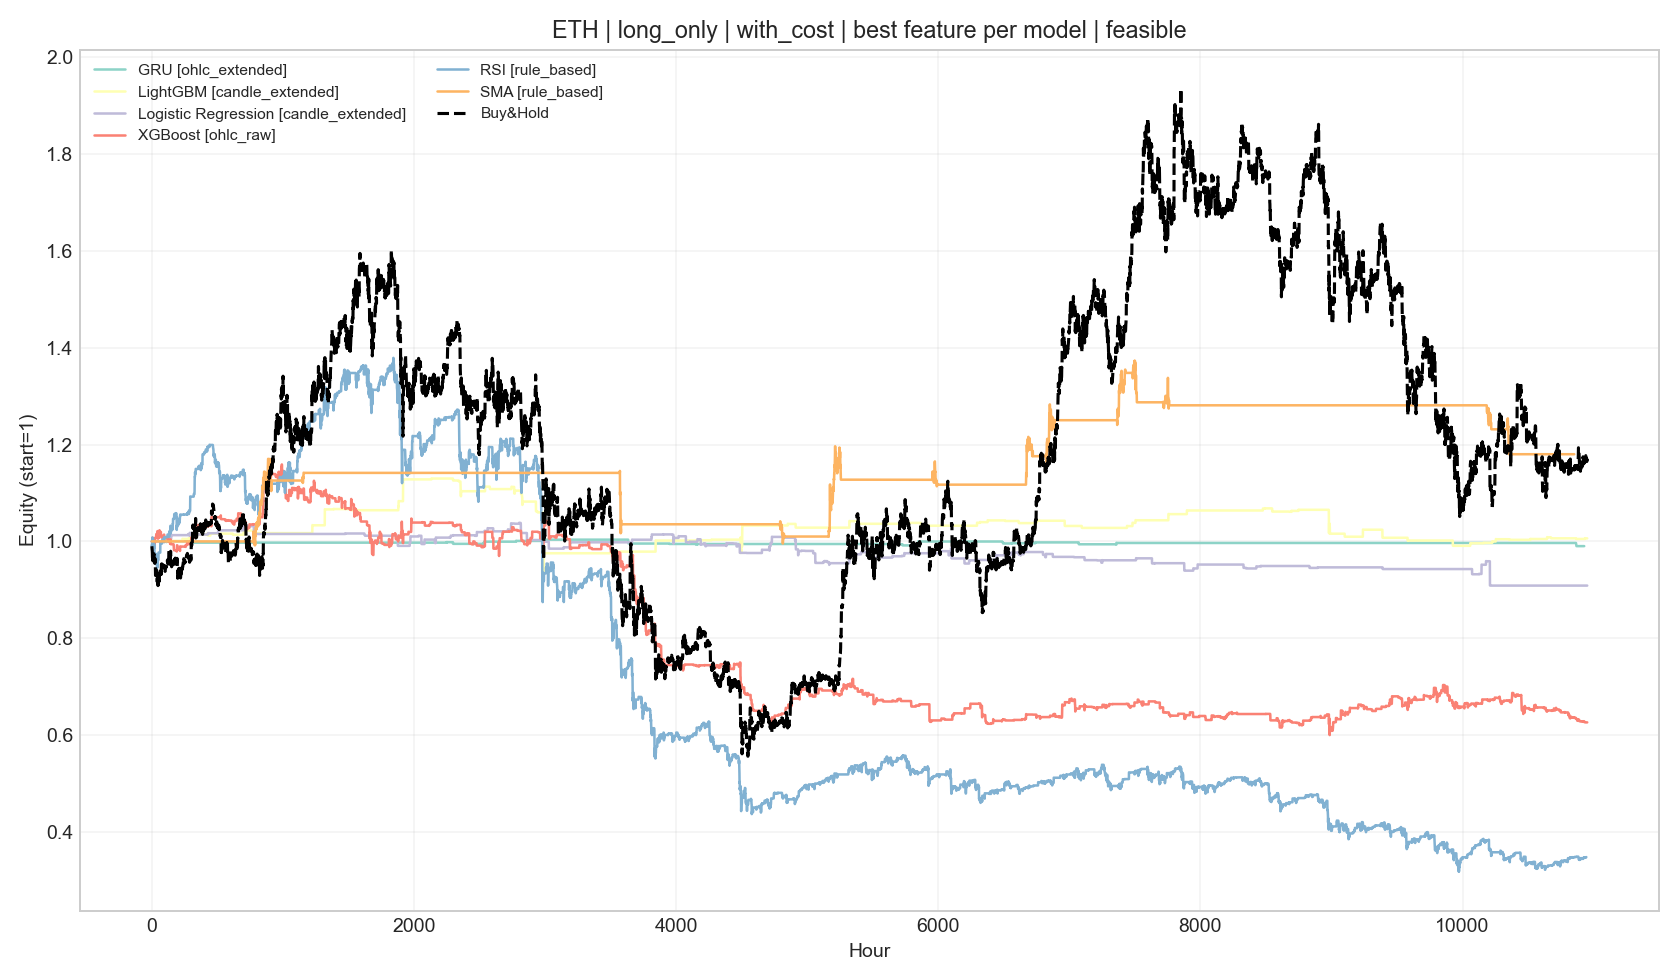
\includegraphics[width=0.9\textwidth]{../result/graph/feasible/ETH/with_cost/long_only/equity_curves_best_feature_per_model_feasible.png}
\caption{ETH long-only equity curves under transaction costs.}
\end{figure}

\begin{figure}[H]
\centering
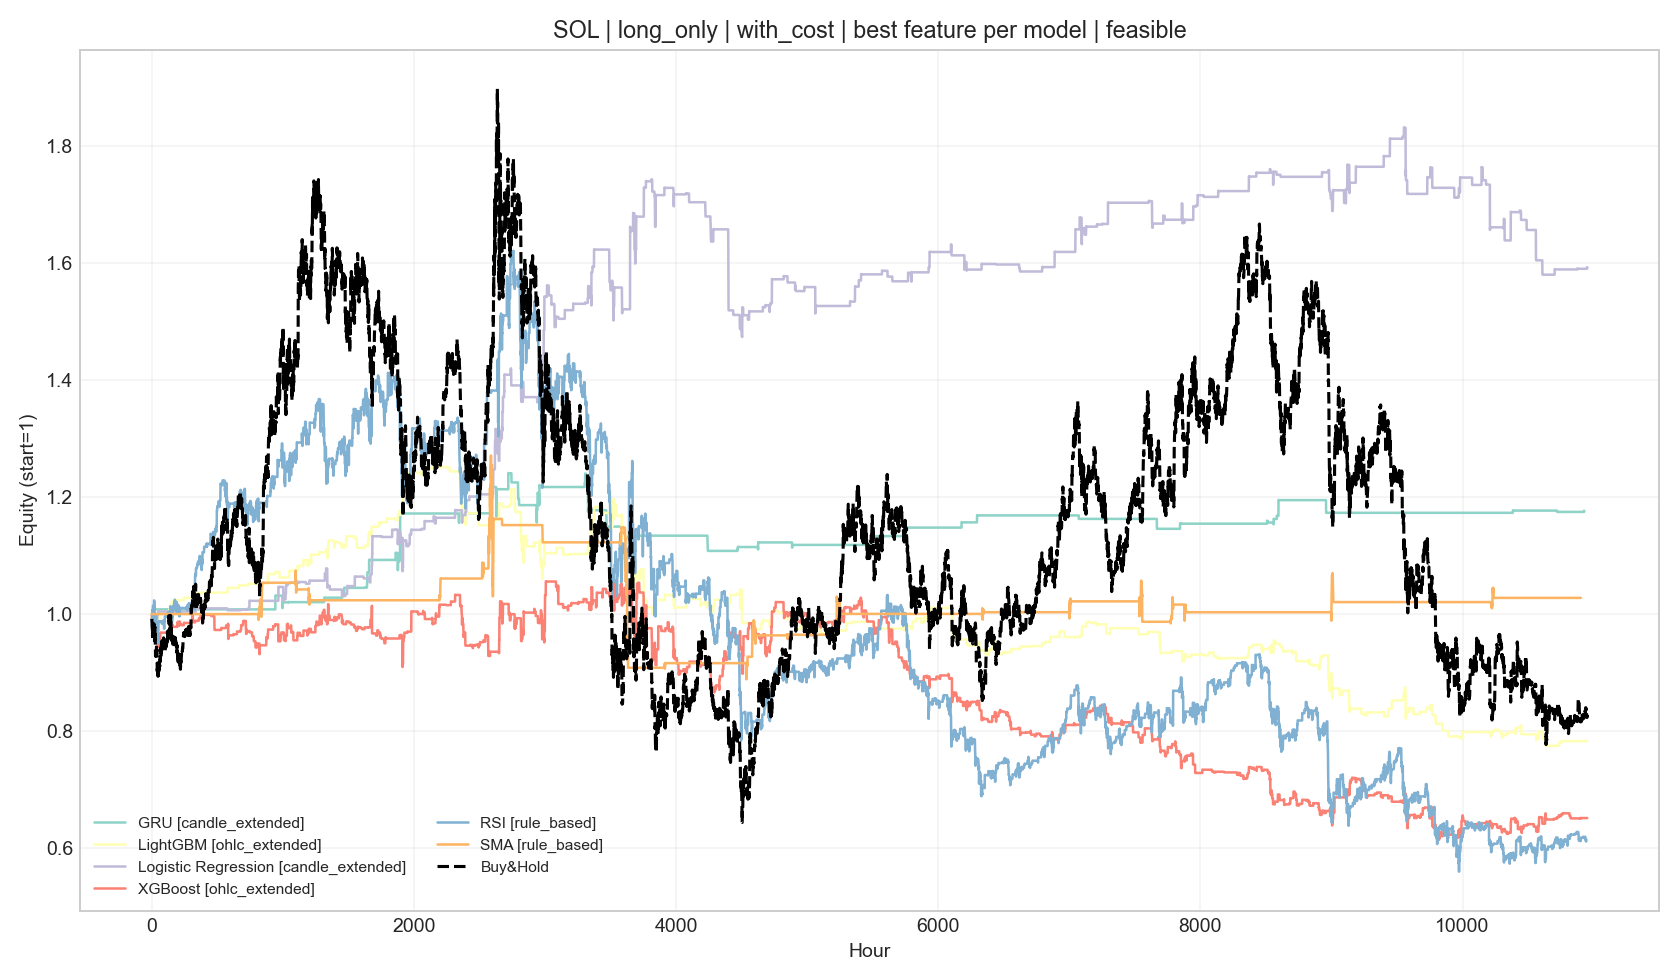
\includegraphics[width=0.9\textwidth]{../result/graph/feasible/SOL/with_cost/long_only/equity_curves_best_feature_per_model_feasible.png}
\caption{SOL long-only equity curves under transaction costs.}
\end{figure}

\begin{figure}[H]
\centering
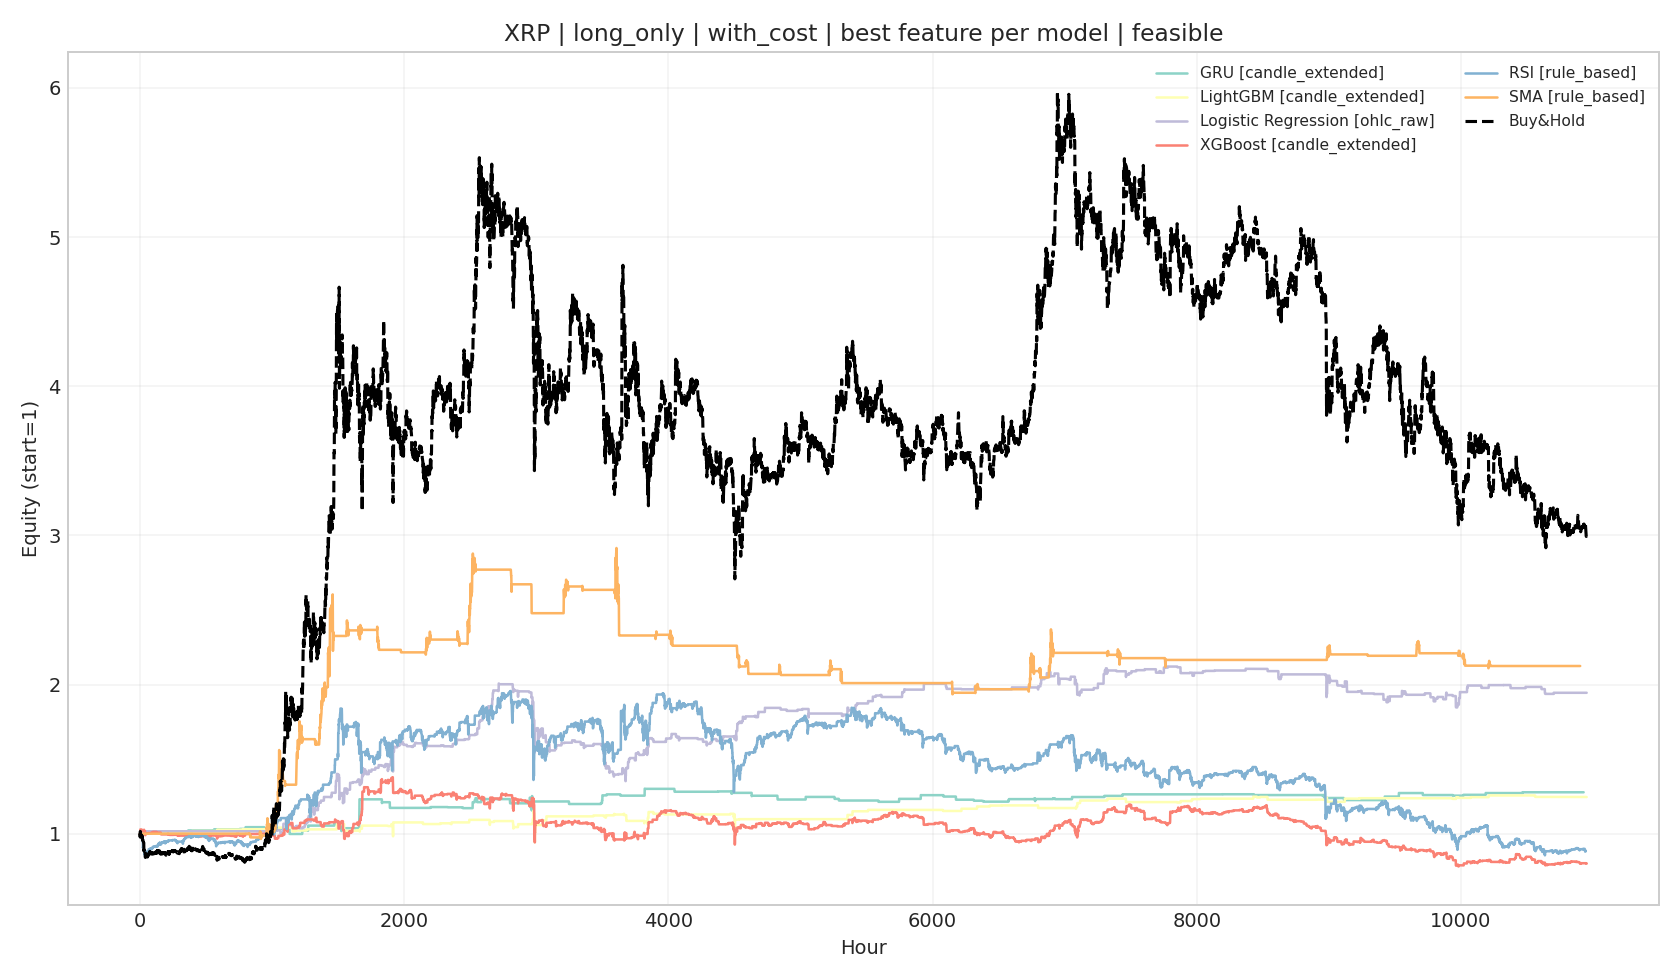
\includegraphics[width=0.9\textwidth]{../result/graph/feasible/XRP/with_cost/long_only/equity_curves_best_feature_per_model_feasible.png}
\caption{XRP long-only equity curves under transaction costs.}
\end{figure}

\subsection{Long-Short With-Cost Equity Curves}

\begin{figure}[H]
\centering
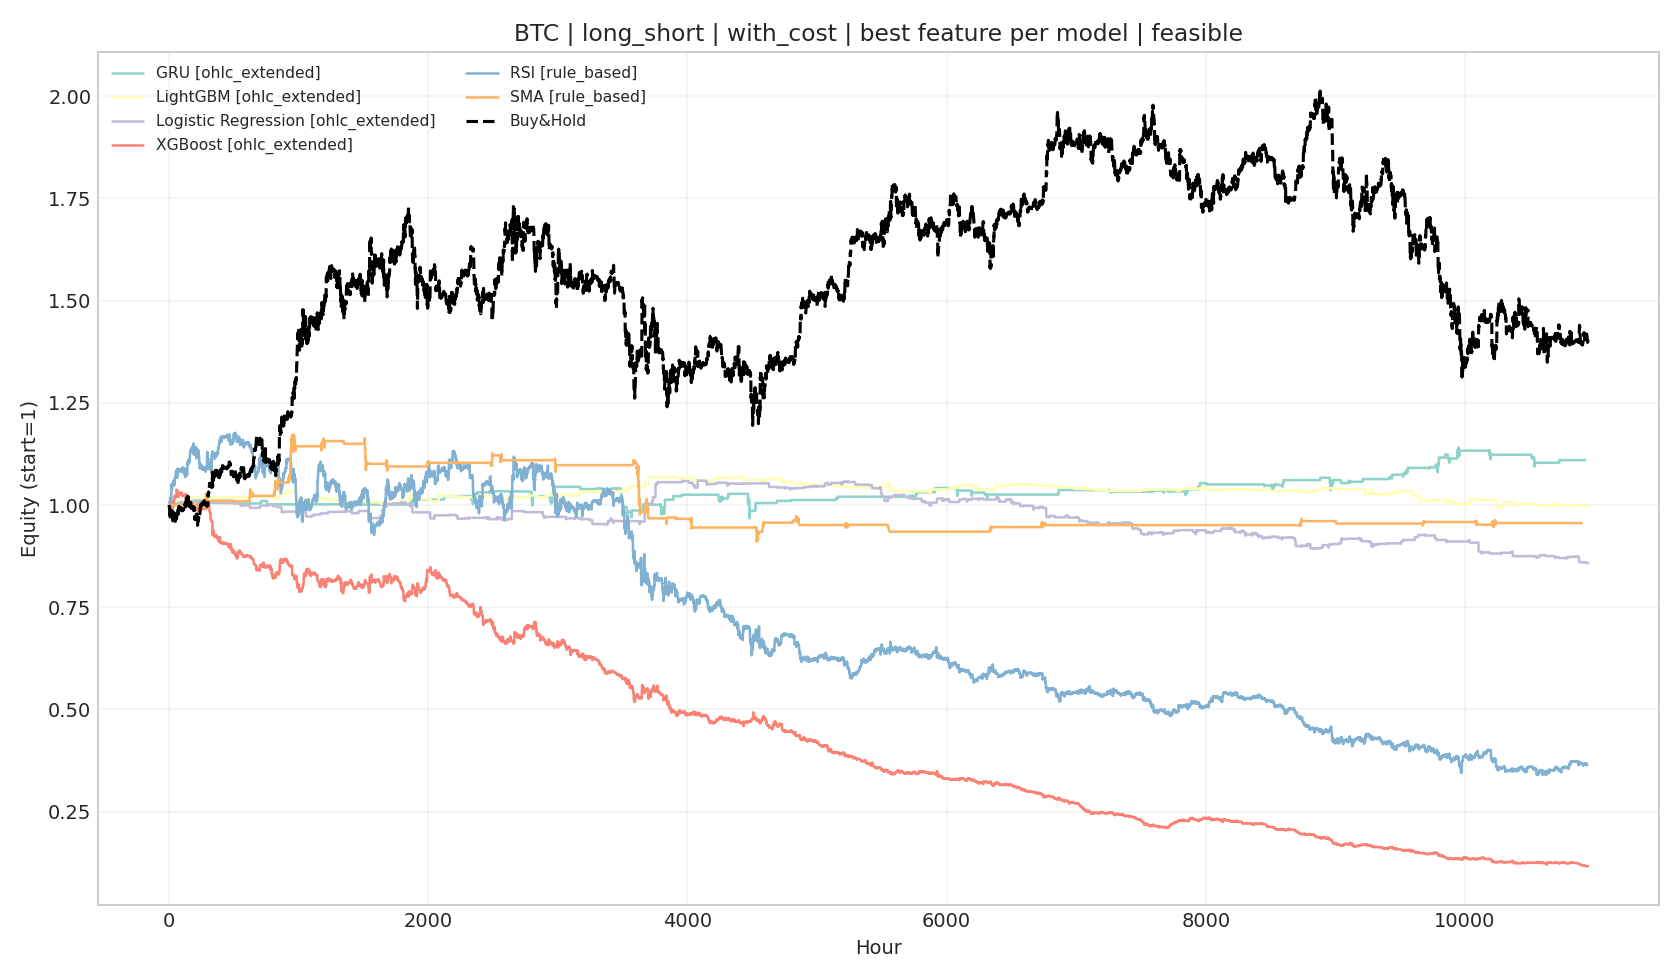
\includegraphics[width=0.9\textwidth]{../result/graph/feasible/BTC/with_cost/long_short/equity_curves_best_feature_per_model_feasible.png}
\caption{BTC long-short equity curves under transaction costs.}
\end{figure}

\begin{figure}[H]
\centering
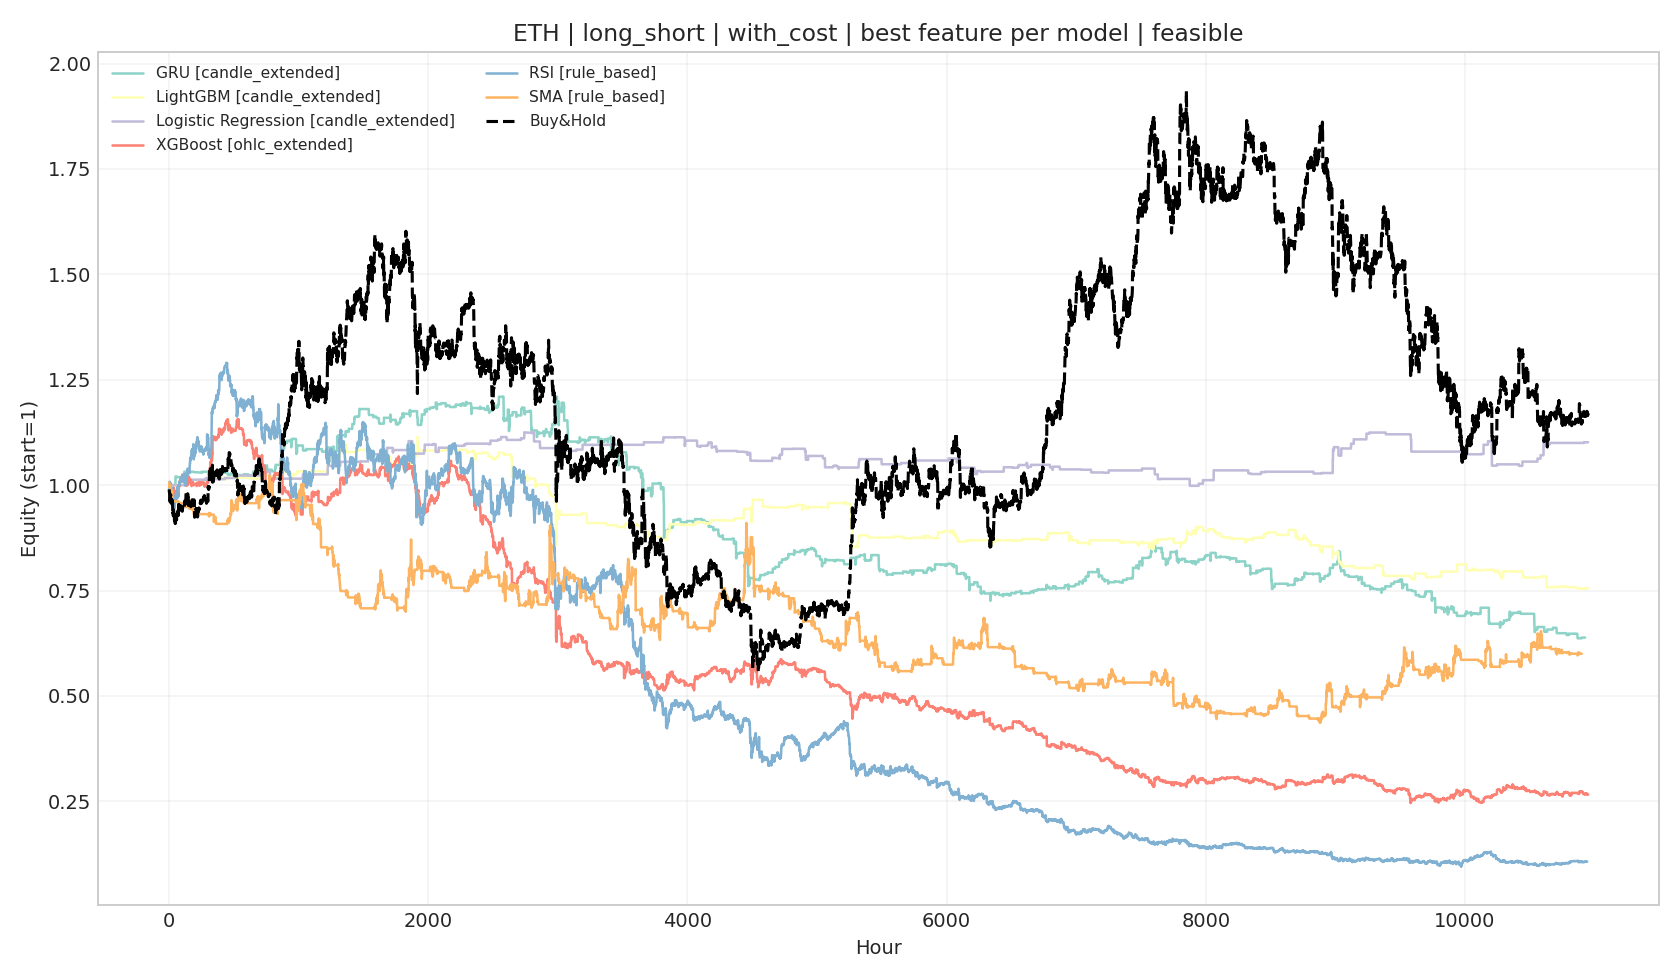
\includegraphics[width=0.9\textwidth]{../result/graph/feasible/ETH/with_cost/long_short/equity_curves_best_feature_per_model_feasible.png}
\caption{ETH long-short equity curves under transaction costs.}
\end{figure}

\begin{figure}[H]
\centering
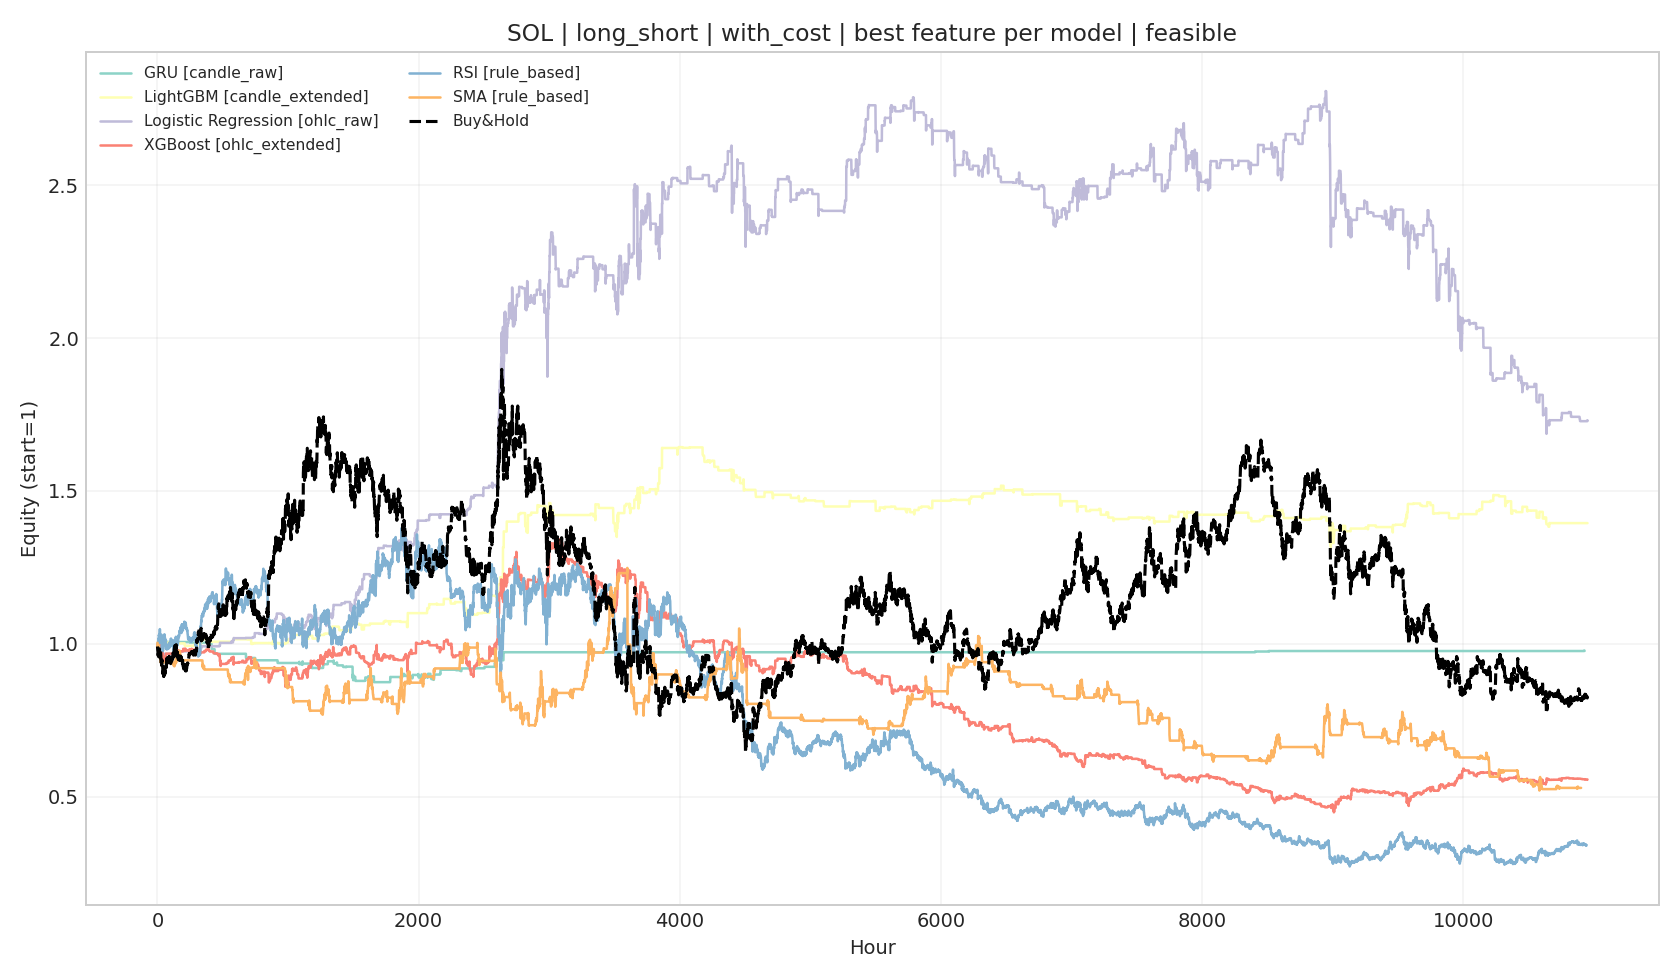
\includegraphics[width=0.9\textwidth]{../result/graph/feasible/SOL/with_cost/long_short/equity_curves_best_feature_per_model_feasible.png}
\caption{SOL long-short equity curves under transaction costs.}
\end{figure}

\begin{figure}[H]
\centering
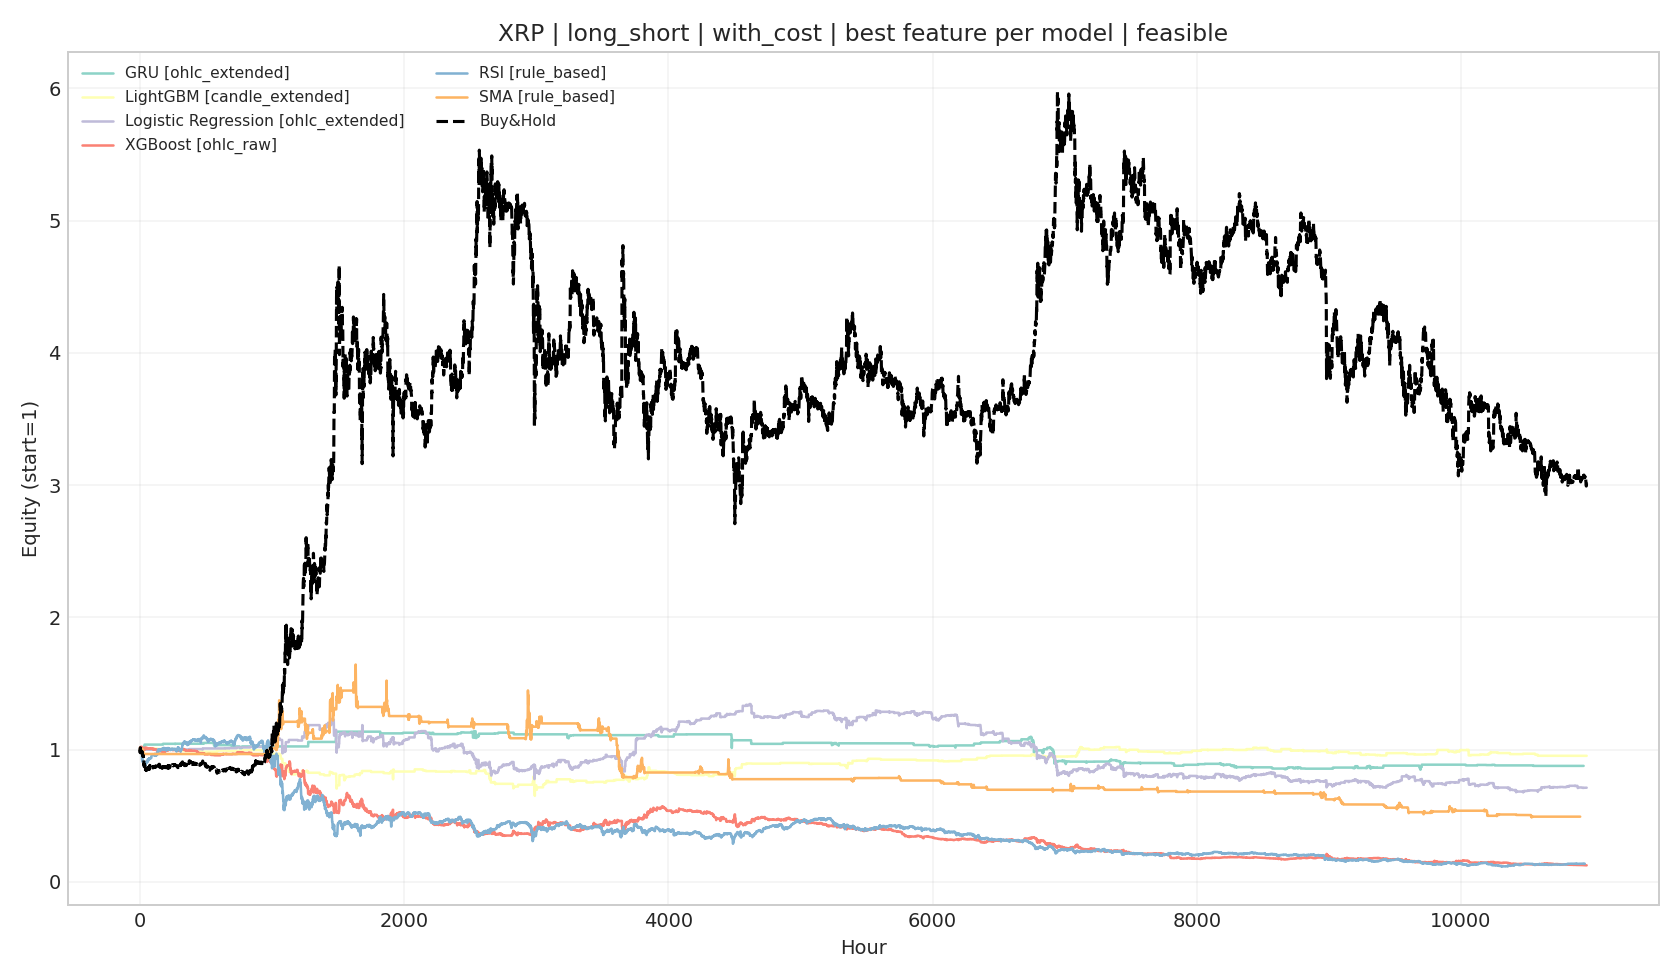
\includegraphics[width=0.9\textwidth]{../result/graph/feasible/XRP/with_cost/long_short/equity_curves_best_feature_per_model_feasible.png}
\caption{XRP long-short equity curves under transaction costs.}
\end{figure}

\subsection{Short-Only With-Cost Equity Curves}

\begin{figure}[H]
\centering
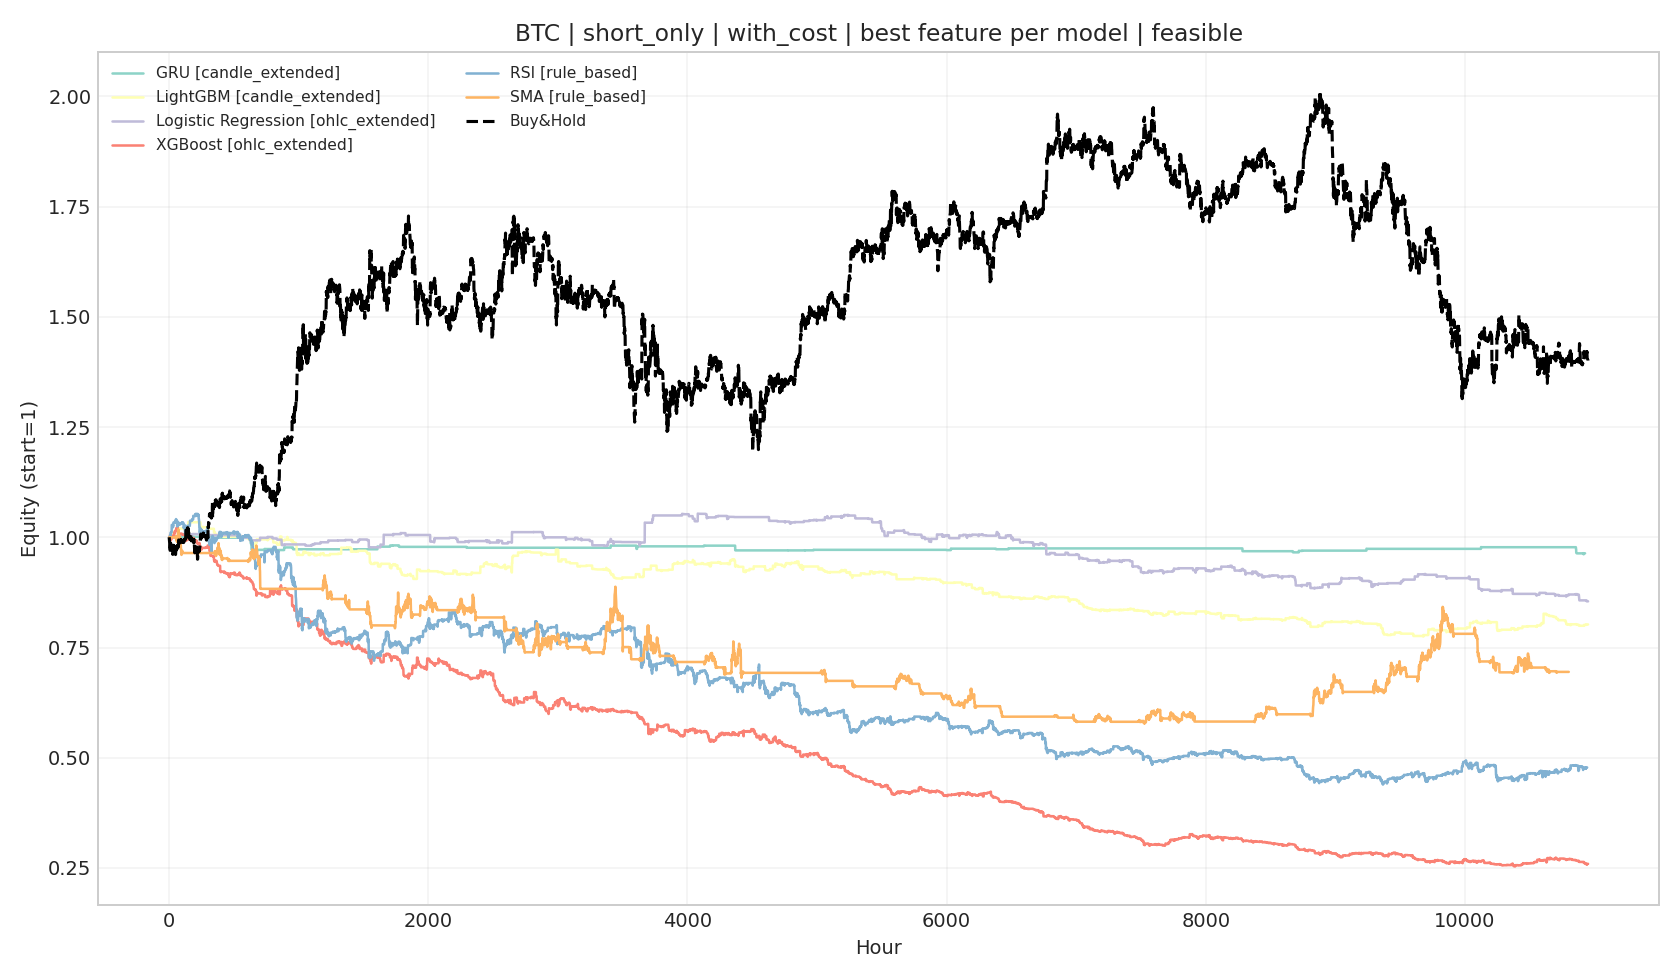
\includegraphics[width=0.9\textwidth]{../result/graph/feasible/BTC/with_cost/short_only/equity_curves_best_feature_per_model_feasible.png}
\caption{BTC short-only equity curves under transaction costs.}
\end{figure}

\begin{figure}[H]
\centering
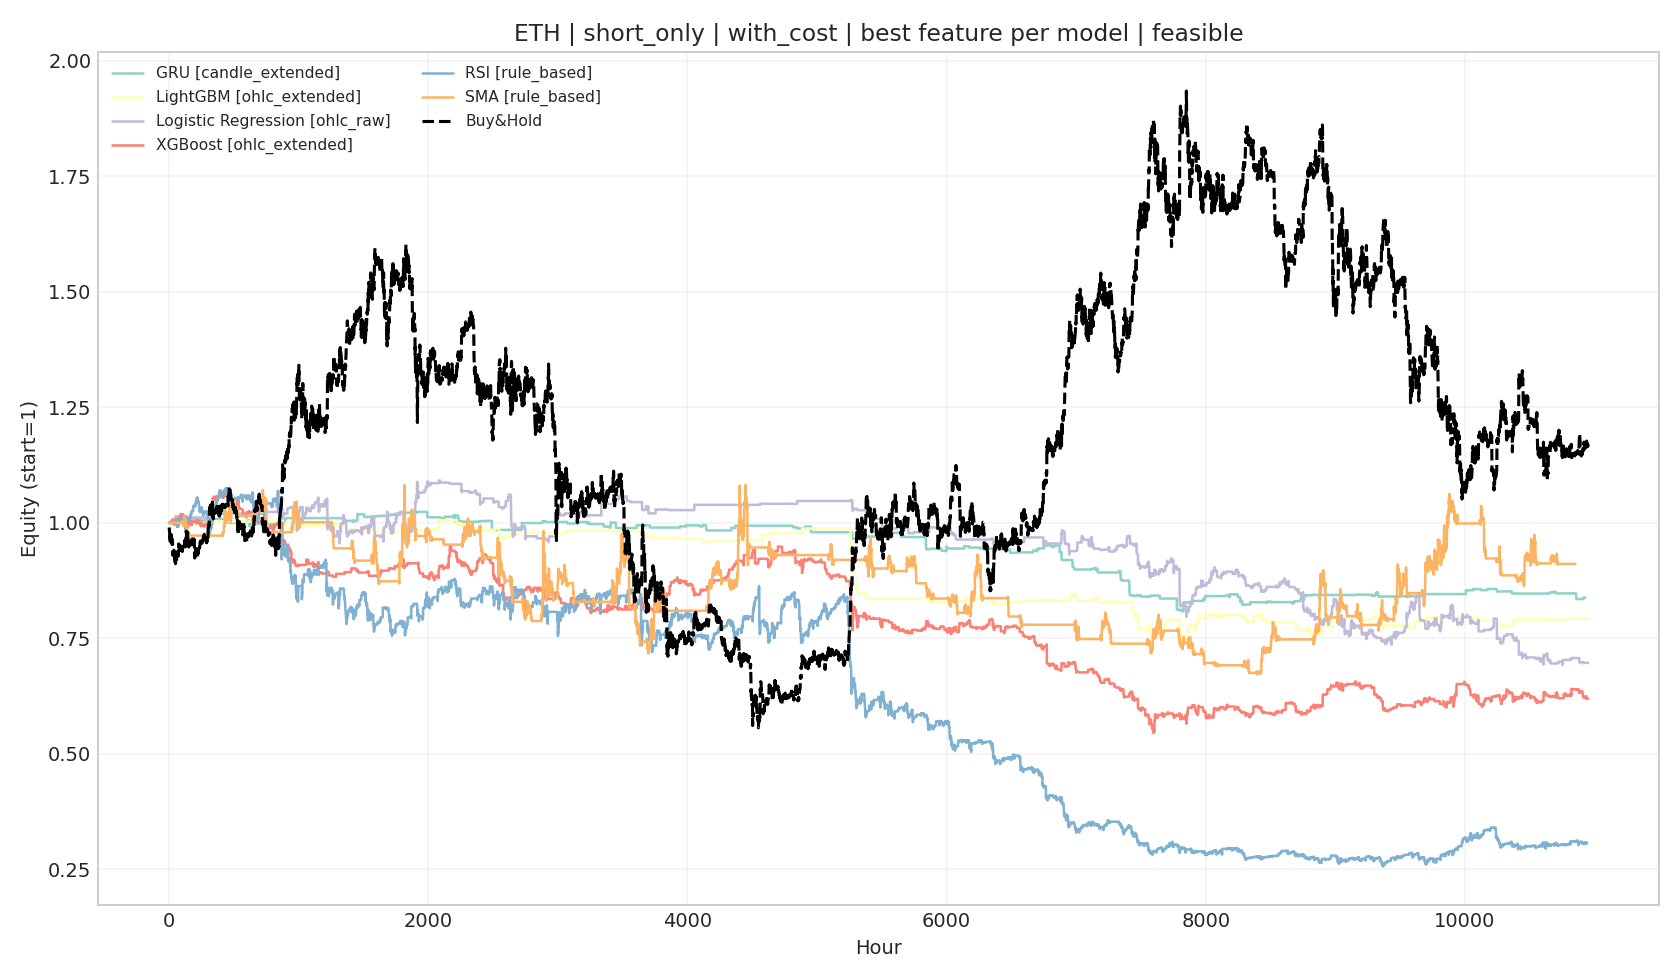
\includegraphics[width=0.9\textwidth]{../result/graph/feasible/ETH/with_cost/short_only/equity_curves_best_feature_per_model_feasible.png}
\caption{ETH short-only equity curves under transaction costs.}
\end{figure}

\begin{figure}[H]
\centering
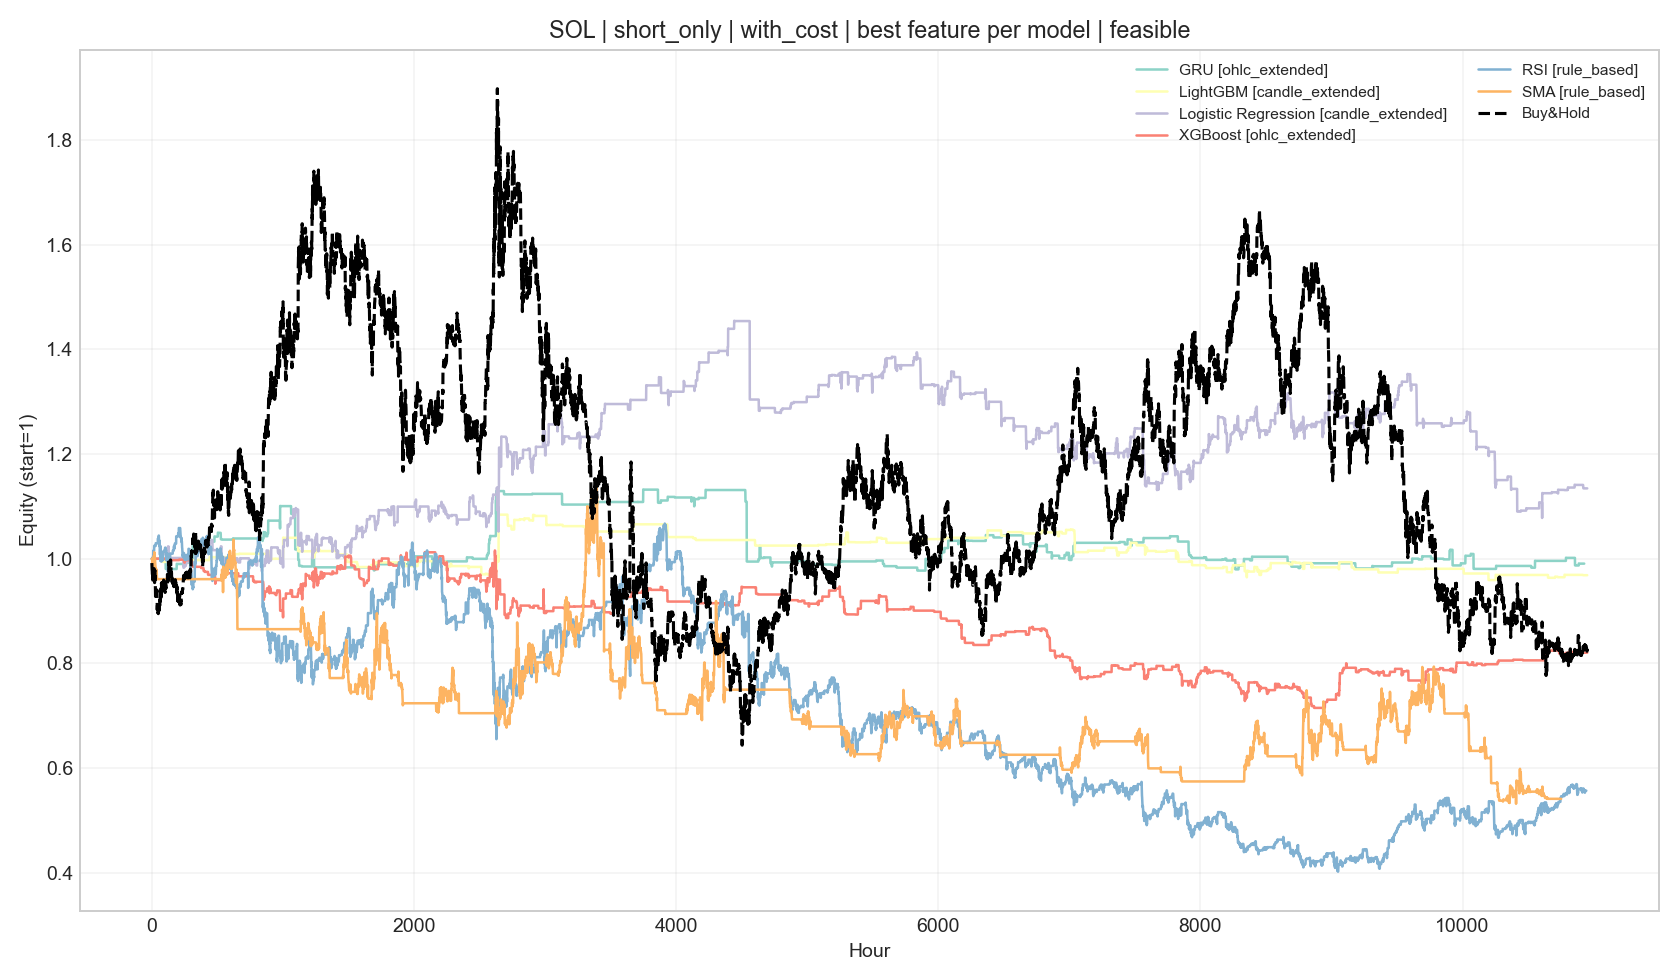
\includegraphics[width=0.9\textwidth]{../result/graph/feasible/SOL/with_cost/short_only/equity_curves_best_feature_per_model_feasible.png}
\caption{SOL short-only equity curves under transaction costs.}
\end{figure}

\begin{figure}[H]
\centering
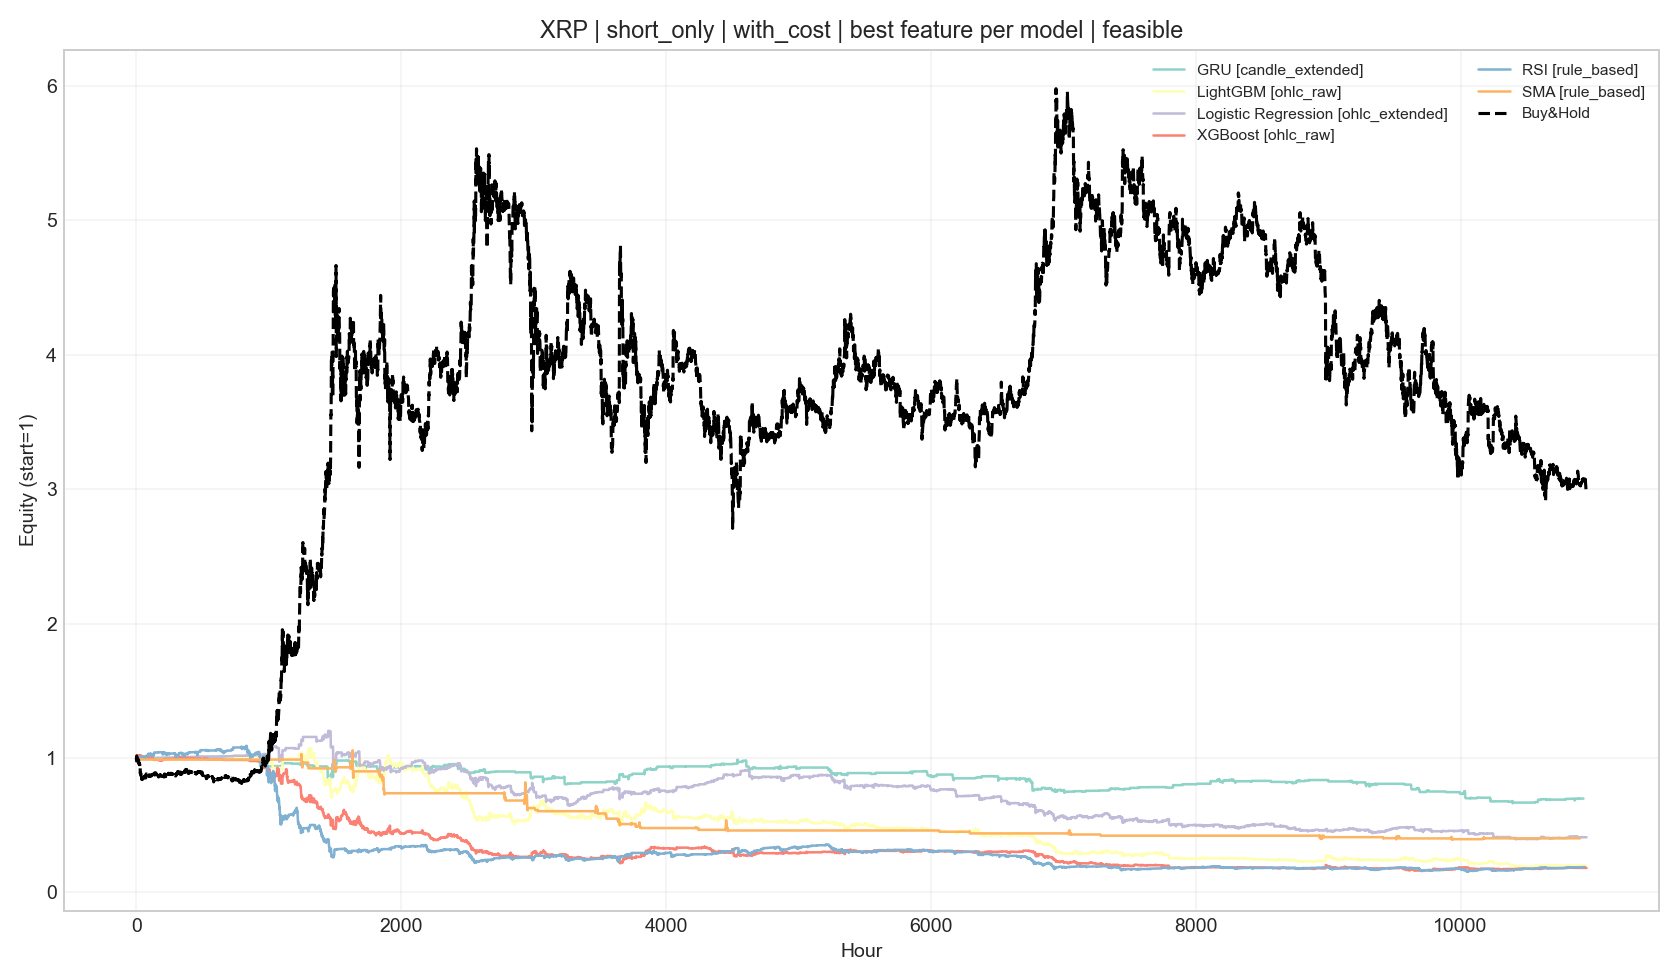
\includegraphics[width=0.9\textwidth]{../result/graph/feasible/XRP/with_cost/short_only/equity_curves_best_feature_per_model_feasible.png}
\caption{XRP short-only equity curves under transaction costs.}
\end{figure}

\clearpage
\section*{Supplementary Rebuttal}
\begingroup
\small
\singlespacing
We summarized the suggestions from the five classmates---1: \texttt{3dkdiz}, 2: \texttt{3eyyuc}, 3: \texttt{3radnt}, 4: \texttt{3sgrqy}, and 5: \texttt{3sskvf}---into 28 concise points below.

\begin{enumerate}[leftmargin=1.5em]
    \item \textbf{Single train/test split}: One fixed historical window may not generalise across market regimes. (by 2, 4, 5) \textit{Response:} admitted as a limitation in the \emph{Limitations} subsection.
    \item \textbf{Regime-conditioned analysis}: Reporting results by regime would strengthen the generalisation claim. (by 2, 3) \textit{Response:} not added in this round; left as future work in \emph{Limitations} and \emph{Future Work}.
    \item \textbf{Binary classification target}: Direction-only prediction ignores return magnitude. (by 2, 3, 4) \textit{Response:} acknowledged as a limitation in \emph{Limitations}.
    \item \textbf{Sharpe formulation and code consistency}: Sharpe definitions were unclear. (mainly by 2) \textit{Response:} fixed in \emph{Evaluation Metrics and Feasibility Rules}, which now states the paper formula and distinguishes annualized Sharpe.
    \item \textbf{Short-only underperformance unexplained}: The consistent weakness of short-only strategies needed interpretation. (by 1) \textit{Response:} fixed in \emph{Feature Representation and Strategy Behaviour}.
    \item \textbf{Tuning asymmetry}: Reviewers thought ML was tuned while SMA/RSI were not. (by 1) \textit{Response:} rebutted in \emph{Rule-Based Technical Heuristics}; SMA and RSI are validation-tuned too.
    \item \textbf{Transaction-cost sensitivity}: A broader fee sweep was suggested. (by 1, 5) \textit{Response:} we keep the Binance-aligned fee design and treat broader sensitivity analysis as beyond this round.
    \item \textbf{Backtest realism}: Slippage, liquidity, and realistic shorting frictions are omitted. (by 3, 4) \textit{Response:} admitted as a limitation in \emph{Limitations}.
    \item \textbf{Precision-first tuning vs Sharpe objective}: The selection objective looked mismatched with the economic objective. (by 4) \textit{Response:} clarified in \emph{Evaluation Metrics and Feasibility Rules} as a deliberate high-confidence signal design.
    \item \textbf{Noisy hourly frequency}: Hourly trading may be noise-heavy and turnover-heavy. (by 3) \textit{Response:} acknowledged in \emph{Sample Period} and \emph{Limitations}.
    \item \textbf{Cluttered equity curves}: The original bundled plots were too crowded. (by 1) \textit{Response:} fixed by moving the figure set to the appendix and using representative per-model curves.
    \item \textbf{Conclusion did not answer the question directly}: The central conclusion was too indirect. (by 1, 5) \textit{Response:} fixed in \emph{Conclusion}.
    \item \textbf{Feature importance analysis absent}: The report did not explain which indicators drive the extended-feature results. (by 1, 3) \textit{Response:} not added; admitted indirectly via the explainability and feature-selection limitations.
    \item \textbf{Rule-based strategy implementation vague}: It was unclear whether long-only, short-only, and long-short applied to SMA/RSI too. (by 5) \textit{Response:} fixed in \emph{Rule-Based Technical Heuristics}.
    \item \textbf{Infeasible configurations not explained}: Excluded configurations needed a principled explanation. (by 5) \textit{Response:} fixed in \emph{Evaluation Metrics and Feasibility Rules}.
    \item \textbf{Literature review too long}: More space should be devoted to interpretation and methodology. (by 5) \textit{Response:} fixed by shortening the literature review and shifting weight to analysis.
    \item \textbf{No README}: The repo previously lacked a clear entry point. (by 1, 2, 3, 4, 5) \textit{Response:} fixed in \texttt{README.md}.
    \item \textbf{Inaccessible GitHub repository}: The original review link was not publicly accessible. (by 1, 2) \textit{Response:} operational issue to be corrected at submission; the repo path is now organized for a public handoff.
    \item \textbf{Redundant notebooks}: Multiple notebooks created ambiguity about the canonical pipeline. (by 1) \textit{Response:} fixed by consolidating the repo around \texttt{project.ipynb}.
    \item \textbf{GRU undocumented}: The most complex model needed clearer documentation. (by 1) \textit{Response:} fixed in \emph{Machine-Learning Models} and the canonical notebook.
    \item \textbf{Messy results output}: The result folders were hard to navigate. (by 4) \textit{Response:} partially fixed by cleaning the repo structure and surfacing the report-facing outputs.
    \item \textbf{Reproducibility failure (GRU)}: Earlier reruns produced different GRU results. (by 4) \textit{Response:} mitigated by global seeding and deterministic TensorFlow settings in \texttt{project.ipynb}; final reported values were then resynchronised with the rerun outputs.
    \item \textbf{No requirements file}: Environment setup was underspecified. (by 1) \textit{Response:} fixed in \texttt{requirements.txt}.
    \item \textbf{No cross-validation}: Rolling or walk-forward validation would provide stronger evidence of stability. (by 3, 5) \textit{Response:} admitted as a limitation in \emph{Limitations}.
    \item \textbf{Class imbalance not addressed}: The report should show whether the labels are materially imbalanced. (by 3) \textit{Response:} fixed with the class-balance note in \emph{Prediction Labelling}.
    \item \textbf{Limited hyperparameter tuning for ML models}: The ML models rely on mostly fixed hyperparameters. (by 3) \textit{Response:} not expanded in this round; this remains a limitation of the submitted design.
    \item \textbf{No feature selection or dimensionality reduction}: Redundancy and multicollinearity may remain in the engineered features. (by 3, 5) \textit{Response:} admitted as a limitation in \emph{Limitations}.
    \item \textbf{No model explainability}: The study does not yet show which features drive predictions. (by 3) \textit{Response:} admitted as a limitation in \emph{Limitations} and \emph{Future Work}.
\end{enumerate}
\endgroup

\end{document}
